\section{Mystery Datensatz}

In diesem Versuchsteil wurden mehrere Datensätze eines unbekannten Ereignisses im Atlasdetektor vorgegeben.
Aufgabe war es, anhand der sichtbaren, markanten Eigenschaften, auf das zu Grunde liegende Ereignis zu schlussfolgern. 
Die Datensätze wurden dabei jedoch so vorselektiert, dass stets mindestens zwei Leptonen ($e$ oder $\mu$) vorhanden waren.
Im Versuch wurde Datensatz 12 verwendet.
Einige Beispielhafte Detektoraufnahmen des Datensatzes sind in Abb. \ref{mysterydata} dargestellt.
Zusätzlich wurden folgende mögliche Ereignisse vorgegeben:
\begin{itemize}
\item $t \overline{t}$
\item $b \overline{b}$
\item ZZ
\item WZ
\item Z $\rightarrow \tau \overline{\tau}$
\item H $\rightarrow \tau \overline{\tau}$
\end{itemize}


Als Ereignis haben wir hier den ZZ-Zerfall identifiziert.
Zur Begründung rekapitulieren wir die möglichen Zerfallskanäle:
Das Top-Quark zerfällt in 96\% aller Fälle in ein Bottom-Quark, ein Lepton und ein Neutrino.
Danach ist der weitere Zerfallsweg, aufgrund des Bottom-Quarks, weitgehend identisch zum $b \overline{b}$ Ereignis.
Da das Bottom-Quark über die starke Wechselwirkung zerfallen kann, muss es bei diesen Ereignis häufige hadronische Schauer geben, die im hadronischen Kalorimeter deutlich zu sehen sein müssten.
Da dies offenbar nicht zu sehen ist (siehe Abb. \ref{mysterydata}), können beide Ereignisse ausgeschlossen werden.

Das Z-Boson kann, unter der Vorgabe dass zwei Leptonen entstehen, hier nur in ein Lepton-Antilepton-Paar zerfallen.
Beim ZZ-Ereignis wäre jedoch daneben noch der Zerfall in ein Neutrino-Antineutrino-Paar möglich.

Dass W-Boson hat leptonische Zerfallskanäle, in Lepton und Antineutrino sowie hadronische in ein Quark und ein Antiquark.
Da das W-Boson eine Ladung besitzt, muss beim WZ Ereignis, aufgrund der Ladungserhaltung, eine überschüssige Ladung vorhanden sein.
Dies wurde in den Datensätzen nicht beobachtet, weshalb auch diese Ereignis ausgeschlossen wurde.
Zusätzlich gegen dieses Ereignis spricht, dass das W-Boson hier einen hadronischen Zerfallsweg besitzen kann.
Da jedoch wie gesagt keine großen hadronischen Schauer zu sehen waren, spricht auch das gegen dieses Ereignis.

Zuletzt betrachten wir die Zerfälle des Z- und Higgs-Bosons in 2 Tauonen.
Tauonen zerfallen entweder in ein leichteres Lepton sowie 2 Neutrinos oder, was bevorzugt geschieht, auf hadronischen Weg.
Da hier jedoch beim Zerfall 2 Leptonen entstehen müssen, ist der hadronische Zerfall ausgeschlossen.
Damit ergeben sich hier als Zerfallsprodukte: 2 Leptonen, 2 Neutrinos und 2 Antineutrinos.
Aufgrund der entstehenden Neutrinos beim Zerfall der Tauonen, sollte hier häufig eine nennswerte fehlende transversale Energie vorhanden sein. 
Da beim ZZ Ereignis Neutrinos nicht unbedingt entstehen müssen, wäre eine Unterscheidung anhand der fehlenden Energie möglich.
Es war auch zu sehen, dass diese in den Daten ab und zu recht hoch und ab und zu quasi nicht vorhanden war, was für das ZZ Ereignis spricht.

Ein zusätzliches Argument für das ZZ Ereignis lässt sich bei Betrachtung der detektierten Myonen sehen.
Da die Zerfallswahrscheinlichkeiten in Elektronen bzw. Myonen gleich sind, würden wir beim Zerfall eines einzelnen $Z$ in $50\%$ der Fälle ein Elektron und 1 Myon erwarten und sonst jeweils 2 Elektronen oder 2 Myonen.
Beim Zerfall zweier $Z$-Bosonen würden wir demzufolge entweder 0, 2 oder 4 Myonen, aber meist (wenn kein $Z$ in ein Neutrinopaar zerfallen ist) vier Jets erwarten.
Tauonen wiederum können nicht in zwei Myonen zerfallen.
Hier würden wir also entweder 0, 1 oder 2 Myonen und stets zwei Jets erwarten.
Ein einzeln Myon wurde in den Ereignissen nicht gefunden, dafür aber einzelne Ereignisse mit vier Myonen und meist zwei oder vier Jets (siehe Abb. \ref{mytserydata}), was wieder für das ZZ Ereignis spricht.

\begin{figure}[h]
\begin{subfigure}{.8\textwidth}
\centering
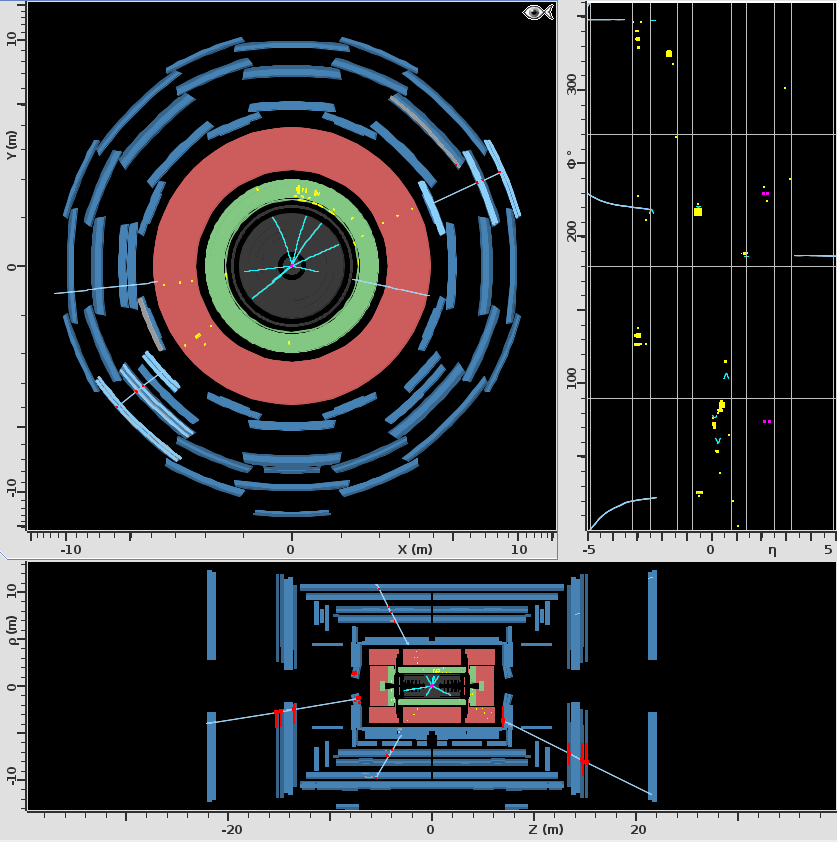
\includegraphics[width=.8\linewidth]{../Pictures/MysteryEvent2.png}
\caption{Ereignis 2}
\end{subfigure}%
\vskip\baselineskip
\begin{subfigure}{.8\textwidth}
\centering
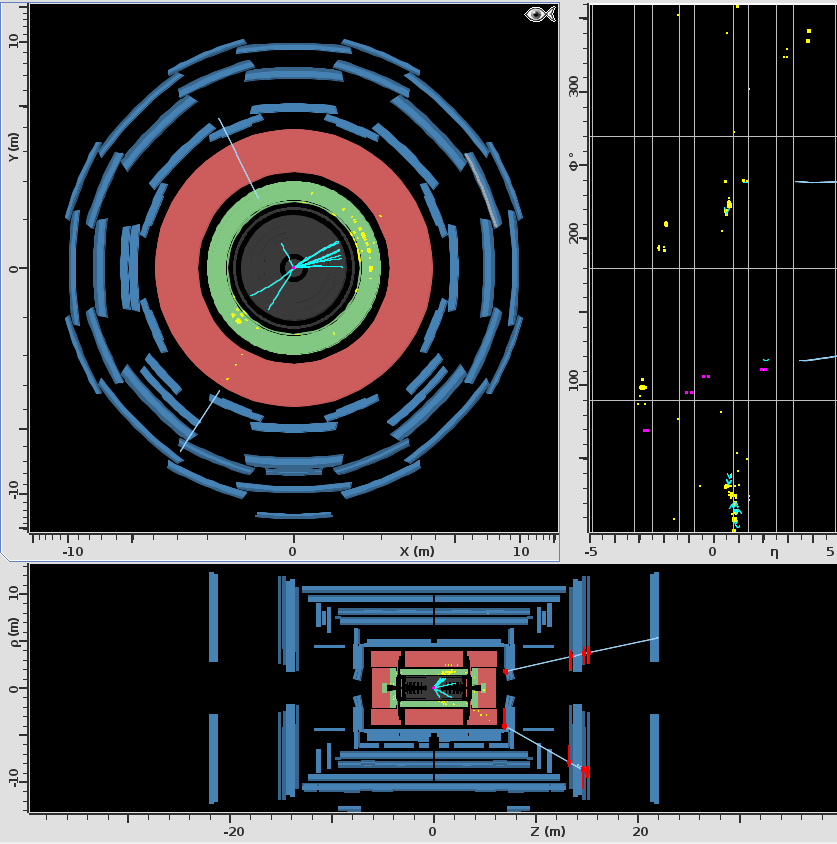
\includegraphics[width=.8\linewidth]{../Pictures/MysteryEvent16.png}
\caption{Ereignis 16}
\end{subfigure}%
\vskip\baselineskip
\begin{subfigure}{.8\textwidth}
\centering
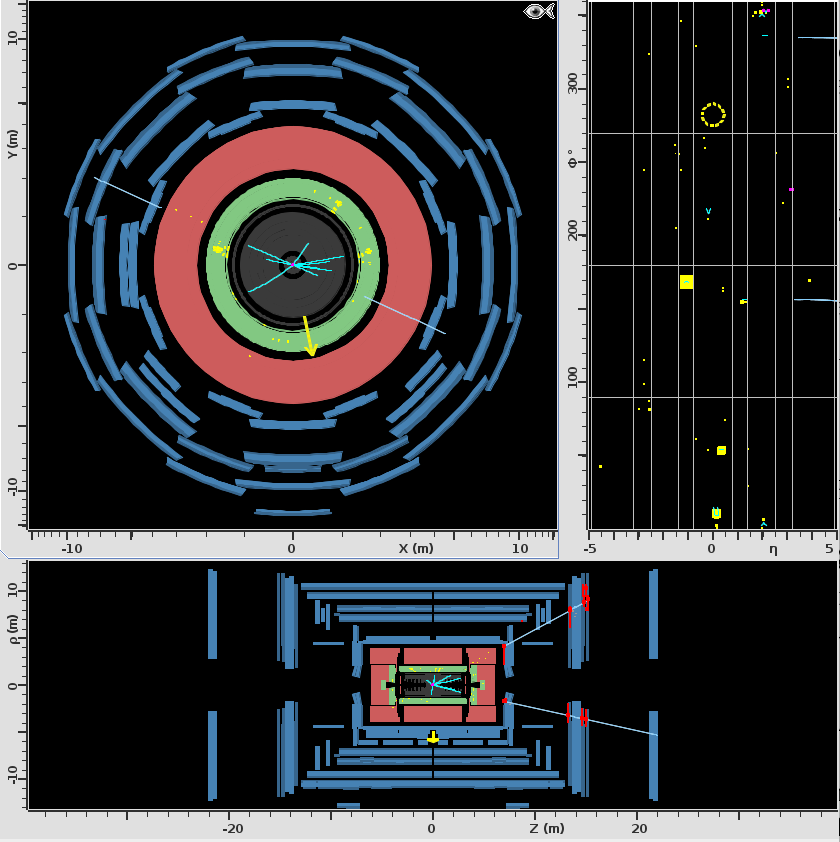
\includegraphics[width=.8\linewidth]{../Pictures/MysteryEvent21.png}
\caption{Ereignis 21}
\end{subfigure}%
\caption{Beispielhafte Ereignisse der Mysterydaten}
\label{mysterydata}
\end{figure}

\clearpage